\documentclass{report}
\usepackage{hyperref}
\usepackage[ngerman]{babel}
\usepackage{amsmath}
\usepackage{amsfonts}
\usepackage{amsthm}
\usepackage{tcolorbox}
\usepackage[a4paper, total={7in, 9in}]{geometry}
\usepackage[font={scriptsize,it}]{caption}
\usepackage{scrextend}
\usepackage{graphicx}
\usepackage{caption}
\usepackage{subcaption}
\usepackage[utf8]{inputenc}
\usepackage[T1]{fontenc}
\DeclareUnicodeCharacter{2212}{-}
\usepackage{verbatim}
\usepackage{tikz}

\tikzset{
  treenode/.style = {shape=rectangle, rounded corners,
                     draw, align=center,
                     top color=white, bottom color=blue!20},
  root/.style     = {treenode, font=\Large, bottom color=red!30},
  env/.style      = {treenode, font=\ttfamily\normalsize},
  dummy/.style    = {circle,draw}
}

\tikzstyle{level 1}=[level distance=3.5cm, sibling distance=3.5cm]
\tikzstyle{level 2}=[level distance=3.5cm, sibling distance=2cm]

% floating figure for column
\newenvironment{Figure}
	{\par\medskip\noindent\minipage{\linewidth}}
	{\endminipage\par\medskip}

\theoremstyle{definition}
\newtheorem{definition}{Definition}

\theoremstyle{example}
\newtheorem*{example}{Example}

\begin{document}

\begin{titlepage}
   \vspace*{\stretch{1.0}}
   \begin{center}
      \Large\textbf{Advanced Software Engineering 2 - FS21}\\
      \large\textit{Pascal Brunner - brunnpa7}
   \end{center}
   \vspace*{\stretch{2.0}}
\end{titlepage}

% Beispiel Bild
%\begin{Figure}
%   \centering
%    \includegraphics[width=150px]{img/BasicTerminologySecKeyCrypto.png}
%        \captionof{figure}{Basic Terminology basierend auf Secret Key Cryptography}
%        \label{fig:Basic Terminology}
%    \end{Figure}

\tableofcontents

\newpage

\chapter{Grundlagen des Software Testens}

\section{Begriffe und Motivation}

\textbf{Definition Testen:} \textit{Der Prozess der aus allen Aktivitäten des Lebenszyklus besteht (sowohl statisch als auch dynamisch), 
die sich mit der Planung, Vorbereitung und Bewertung eines Softwareproduktes und dazugehöriger Arbeitsergebnisse befassen. Ziel des Prozesses ist sicherzustellen, 
dass diese allen festelegten Anforderungen genügen, dass sie ihren Zweck erfüllen und etwaige Fehlzustände zu finden}\\

\textbf{Fehlerwirkung / Fehlfunktion / äussere Fehler / Ausfall} (engl. failure): \text{Ein Ereignis in welchem eine Komponente oder ein System eine geforderte Funktion nicht im spezifizierten Rahmen ausführt (nach ISO 24765)}\\

\textbf{Fehlerzustand} (engl. fault, defect, bug): \textit{Defekt (innerer Fehlerzustand) in einer Komponente oder einem System, der eiene geforderte Funktion des Produkts beeinträchtigen kann, z.B. inkorrekte Anweisung oder Datendefinition}\\

\textbf{Fehlhandlung} (engl. Error): \textit{Die menschliche Handlung, die zu einem falschen Ergebnis führt (nach IEEE 610)}\\

\begin{Figure}
   \centering
    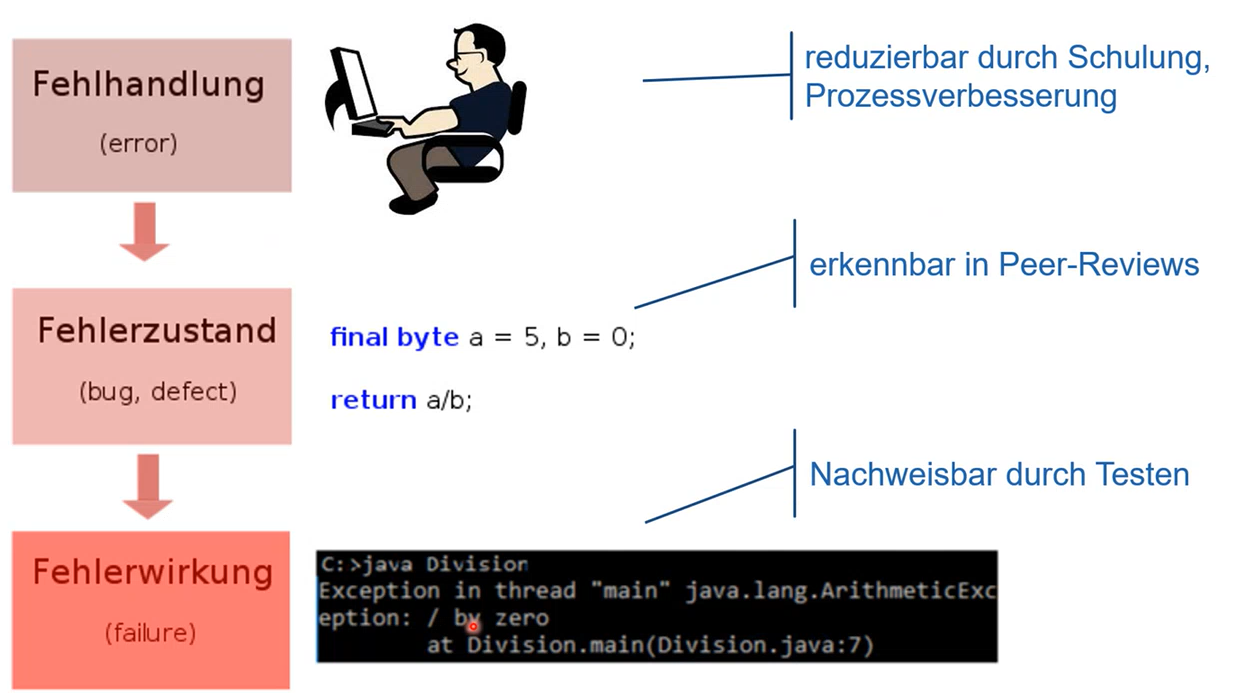
\includegraphics[width=150px]{img/Fehlerbegriffe.png}
        \captionof{figure}{Abbildung der Fehlerbegriffe}
        \label{fig:Fehlerbegriffe}
    \end{Figure}

\textbf{Fehlermaskierung} (engl. defect masking): \textit{Ein Umstand, bei dem ein Fehlerzustand die Aufdekcung eines anderen verhindert (nach IEEE 610)}

\begin{Figure}
   \centering
    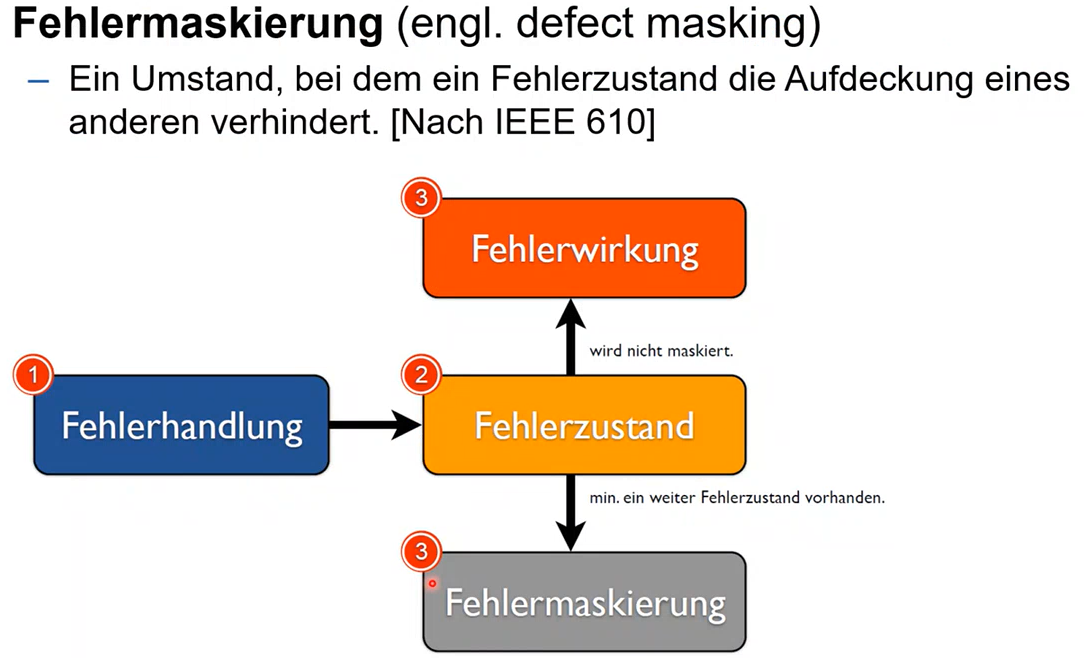
\includegraphics[width=150px]{img/Fehlermaskierung.png}
        \captionof{figure}{Abbildung der Fehlermaskierung}
        \label{fig:Fehlermaskierung}
    \end{Figure}

    \begin{Figure}
      \centering
       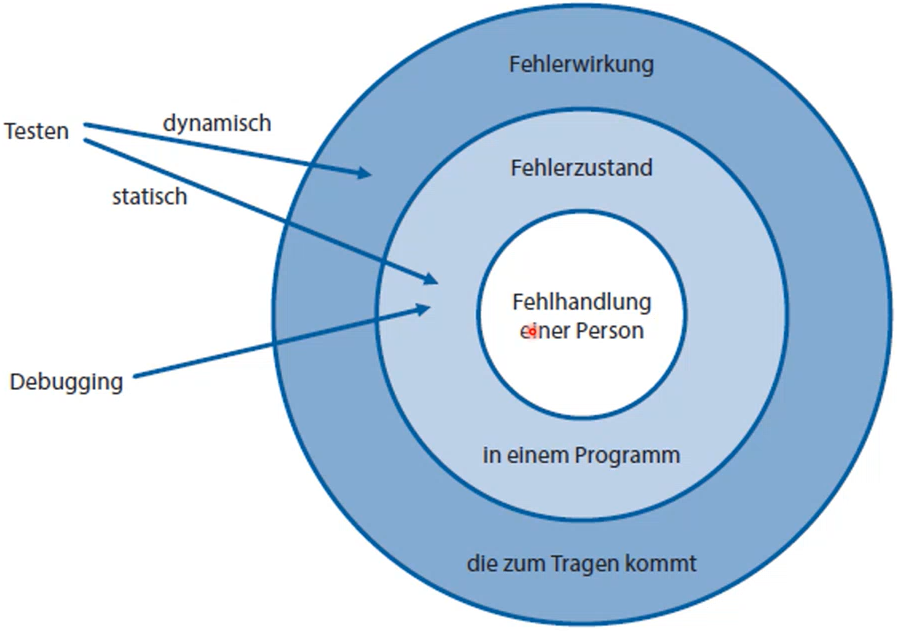
\includegraphics[width=150px]{img/ZusammenhangFehler.png}
           \captionof{figure}{Zusammenhang der Fehler}
           \label{fig:ZusammenhangFehler}
       \end{Figure}

\textbf{False-positive Result}: Testergebnis zeigt Fehlerwirkung, obwohl der Fehlerzustand bzw. die Ursache für die Fehlerwirkung nicht im Testobjekt liegt\\

\textbf{false-negative Result}: Testergebnis zeigt keine Fehlerwirkung, obwohl die Tests diese hätten aufdecken sollen\\
$\rightarrow$ Bei jeder Auswertung von Testergebnissen ist somit zu beachten, ob eine der beiden Möglichkeiten vorliegt\\

\textbf{true-positive result}: Fehlerwirkung durch den Testfall aufgedeckt\\

\textbf{true-negative Result}: erwartetes Verhalten bzw. Ergebnis des Testobjekts mit dem Testfall nachgewiesen

\subsection{Testbegriffe}
Um den Defekt zu korrigieren muss der Defekt lokalisiert werden. Bekannt ist die Wirkung aber nicht die genaue Stelle.\\
\textbf{Fehlerbereinigung, Fehlerkorrektur} (engl. Debugging): Debugging und Testen sind vers. Dinge:
\begin{itemize}
   \item \textbf{Dynamische Tests} können Fehlerwirkung zeigen, die durch Fehlerzustände verursacht werden
   \item \textbf{Debugging} ist eine Entwicklungsaktivtität, die die Ursache (den Fehlerzustand) einer Fehlerwirkung identifiziert, analysiert und entfernt
\end{itemize}


\textbf{Ziele des Testens}
\begin{itemize}
   \item Qualititative Bewertung von Arbeitsergebnisse wie Anforderungsspezifikation, User Stories, Design und Programmtext
   \item Nachweiss, dass alle spez. Anforderung vollständig umgesetzt sind
   \item Vertrauen in die Qualität
   \item Höhe des Risikos bei mangelnder Qualität der Software kann durch Aufdeckung von Fehlerwirkungen verringert werden
\end{itemize}

\textbf{Unsystematischer Test}
\begin{itemize}
   \item Laufversuch: der Entwickler testet
   \subitem Entwickler übersetzt, bindet und startet ein Programm
   \subitem Läuft das Programm nicht oder sind Ergebnisse offensichtlich falsch wird Debugging betrieben
   \subitem Der Test ist beendet wenn das Programm läuft und Ergebnisse vernünftig aussehen
   \item Wegwerf-Test: Testen ohne Systematik
   \subitem Jemand probiert das Programm mit vers. Eingabedaten aus
   \subitem Fallen Ungereimtheiten auf, wird eine Notiz gemacht
   \subitem Der Test endet, wenn der Tester findet, es sei genug getestet 
\end{itemize}


\subsection{Systematischer Test}

\begin{itemize}
   \item Test ist geplant
   \item Programm wird gemäss Testvorschrifft ausgeführt
   \item Ist-Resultat wird mit Soll-Test überprüft
   \item Testergebnisse werden dokumentiert
   \item Fehlersuche und -behebung erfolgen separat
   \item Nicht bestandene Test werden wiederholt
   \item Test endet, wenn vorher definierte Testziele erreicht sind
   \item Die Testspezfiikation wird laufend aktualisiert
\end{itemize}


\textbf{Ziele des systematischen Testens}
\begin{itemize}
   \item Reproduzierbarkeit
   \item Planbarkeit
   \item Wirtschaftlichkeit
   \item Risiko- und Haftungsreduktion
\end{itemize}

\section{Testartefakten}
\begin{Figure}
   \centering
    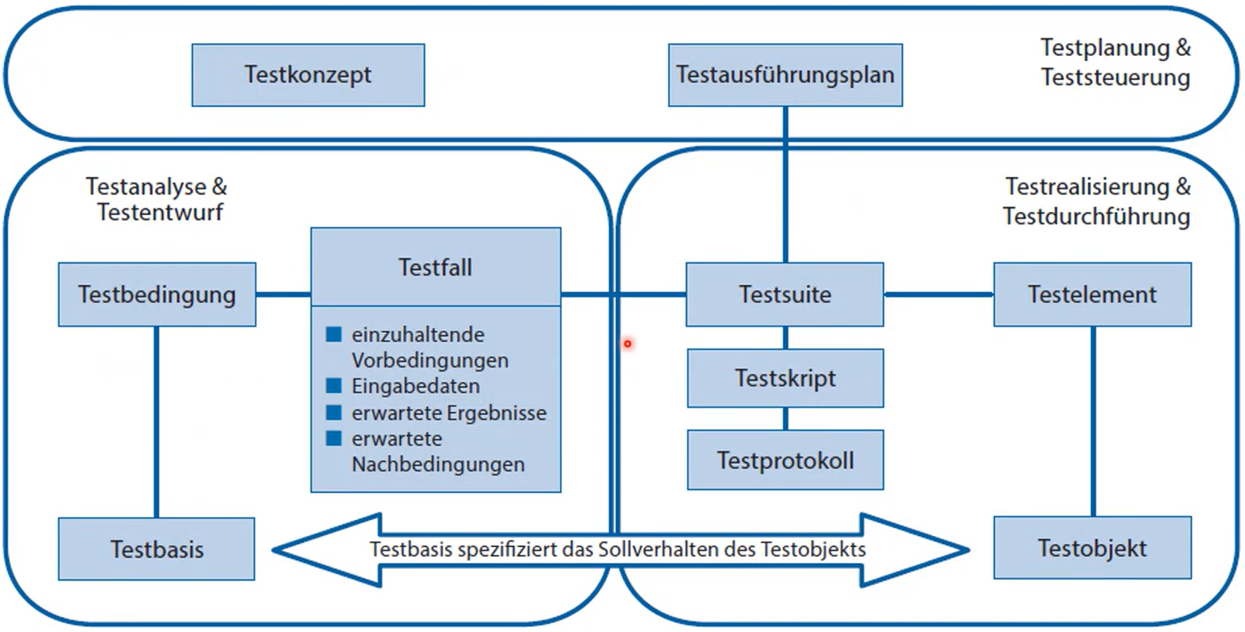
\includegraphics[width=150px]{img/Testartefakte.png}
        \captionof{figure}{Uebersicht der Testartefakten und ihre Beziehungen}
        \label{fig:Testartefakte}
\end{Figure}

\section{Aufwand}
\begin{itemize}
   \item Programm vollständig zu testen ist in der Praxis nicht möglich 
   \item 25-50 Prozent des Entwicklungsaufwands
   \item Testintensität und umfang in Abhängigkeit mit dem Risiko und Kritikalität
   \item 2/3 des Testaufwands können auf Komponententests entfallen
   \item Immer mit beschränkter Ressourcens
\end{itemize}

\section{Grundsätze}
\begin{itemize}
   \item Möglichst frühzeitig alle Beteiligten beiziehen
   \item Beteiligen sich Tester an der Prüfung der Anforderung können Unklarheiten und Fehler in der Arbeitsprodukten aufgedeckt und behoben werden
   \item Die enge Zusammenarbeit von Testern mit Systemdesiger kann das Verständnis für jede Partei für das Design und des Tests erheblich verbessern
   \item Arbeiten Entwickler und Tester während der Codeerstellungs zusammen, kann das Verständnis beidseitig verbessert werden
   \item Wenn Tester die Software vor deren Freigabe verifizieren und validieren können weitere Fehlerzustände erkannt und behoben werden
\end{itemize}

\begin{enumerate}
   \item Testen zeigt die Anwesenheit von Fehlerzuständen
   \item Vollständies Testen ist nicht möglich
   \item Frühes Testen spart Geld und Zeit 
   \item Häufung von Fehlerzustände $\rightarrow$ Taucht in einem Modul ein Fehler auf, gibt es eine hohe Wsk dass noch weitere Fehler sich befinden
   \item Vorischt vor dem Pestizid-Paradox $\rightarrow$ nur wiederholen bringen keinen Mehrwert, Testfälle sind zu prüfen, zu aktualisieren und zu modifizieren
   \item Testen ist kontextabhängig
   \item Trugschluss: Keine Fehler bedeutet ein brauchbares System
\end{enumerate}

\chapter{Testprozess}
Ein Testprozess wird in der Regel folgende Aktivitäten umfassen (ISO-Norm 29119-2):
\begin{itemize}
   \item Testplanung
   \item Testüberwachung und -steuerung
   \item Testanalyse
   \item Testentwurf
   \item Testrealisierung
   \item Testdurchführung
   \item Testabschluss
\end{itemize}
$\rightarrow$ Diese Aktivitäten werden z.T. zeitlich überlappend oder parallel ausgeführt. Der Testprozess ist für jede Teststufe geeignet zu gestalten (Tailoring für ein Projekt)

\section{Testplanung}
\begin{itemize}
   \item Umfangreiche Aufgabe sollte so früh wie möglich begonnen werden
   \item Aufgaben und Zielsetzung der tests müssen festelegt werden, genau wie die Ressourcen
   \item Entsprechende Festlegungen im Testkonzept
   \subitem Testziele
   \subitem Teststrategie
   \subitem Testaktvitäten
   \subitem Ressourcen
   \subitem Testbedingungen und Testbasis
   \subitem Metriken
   \subitem Risiken
   \item Teststrategie bildet der rote Faden 
\end{itemize}

\subsection{Testüberwachung und Teststeuerung}
\begin{itemize}
   \item Die Testüberwachung und Teststeuerung umfasst
   \subitem fortwährende Beobachtung der aktuell durchgeführten Testaktvitäten im Vergleich zur Planung
   \subitem Berichterstattung der ermittelten Abweichungen und die Durchführung der notwendigen Aktivitäten um die Ziele zu erreichen
   \item Basis für Testüberwachung und -steuerung sind Endekriterien für jeweilige Testaktiväten und -aufgaben
\end{itemize}

\subsection{Testanalyse}
Bei der Testanalyse geht es darum, zu ermitterln, was genau zu testen ist
\begin{itemize}
   \item Testbasis prüfen
   \item Dokumente analysieren
   \item Testobjekt selbst prüfen
   \item Berichte heranziehen
   \item Grundlage ist die Testbasis
   \item Priorisierung der Testbedingungen
   \item bidirektionale Rückverfolgung sollte sichergestellt werden (traceability)
\end{itemize}

\subsection{Testentwurf}
Bei Testentwurf geht es darum, festzulegen, wie getestet wird
\begin{itemize}
   \item Spezifikation von abstrakten und konkreten Testfällen
   \item Identifizierung benötigter Testdaten
   \item Ausgangssituation (Vorbedingung)
   \item Randbedingungen
   \item Ergebnisse bzw. welches Verhalten erwartet wird
   \item Sollergebnis
\end{itemize}

\subsection{Testrealisierung}
Abschliessende Vorbereitung aller notwendigen Aktivitäten
\begin{itemize}
   \item Erstellung der Testmittel
   \item Testrahmen programmiert und Testumgebung installiert
   \item Abstrtakte Testfälle sind zu konkretisieren
   \item Testfälle sind zweckmässigerweise zu Testsuiten gruppiert
   \item automatisierte Testskripts
\end{itemize}

\subsection{Testdurchführung}
Umfasst die konkrete Ausführung der Tests und deren Protokollierung
\begin{itemize}
   \item Ausführung von Testabläufen unter Einhaltung des Testplans
   \item Nachvollziehbarkeit und Reproduzierbarkeit
   \item Vergleich Ist-Soll
   \item Fehlerwirkungen oder Abweichungen festhalten
\end{itemize}

\subsection{Testabschluss}
\begin{itemize}
   \item letzte Aktivität im Testprozess
   \item Für Ermittlung von Metriken sollen Testwerkzeuge eingesetzt werden
   \item unterschiedliche Zeitpunkte für Testabschluss
   \item Testabschlussbericht ist zu erstellen
   \subitem Fasst alle Testaktvitäten und -ergebnisse zusammen
   \subitem wird allen Stakeholdern zur Verfügung gestellt
   \subitem Testmittel sind zu archivieren
\end{itemize}

\section{Psychologie des Testens}
\begin{itemize}
   \item Irren ist menschlich
   \item Soll der Entwickler sein eigenes Programm testen?
   \subitem Blindheit gegenüber eigenen Fehler
   \subitem hat hingegen keine Einarbeitungszeit
   \item Drittperson / Tester
   \subitem ist unvoreingenommen
   \subitem Einarbeitung notwendig 
   \subitem Test-Know-how notwendig, bringt ein Tester jedoch mit
   \item Stufen der Abhängigkeit (von niedrig nach hoch)
   \subitem Entwickler selbst
   \subitem Kollegen des Entwicklers
   \subitem Personen anderer Abteilung
   \subitem Person anderer Organisation
   \item Aufteilung ist produkt- bzw. projektabhängig
   \item richtige Mischugn und Ausgewogenheit zwischen unabhängiger Tests und Entwicklertests 
   \item Fehlerwirkungen mitteilen
   \item Reproduzierbarkeit ist wichtig
   \item Eindeutige Anforderungen, präzise Spezifikation
   \item Förderlich für die Zusammenarbeit zw. Tester und Entwickler ist die gegenseitige Kenntnis der Aufgaben
\end{itemize}

\chapter{Testen im Softwareentwicklungslebenszyklus}

\section{Sequentielle Entwicklungsmodelle}
Eines der bekanntestens Modellen ist das Wasserfallmodell

\begin{Figure}
   \centering
    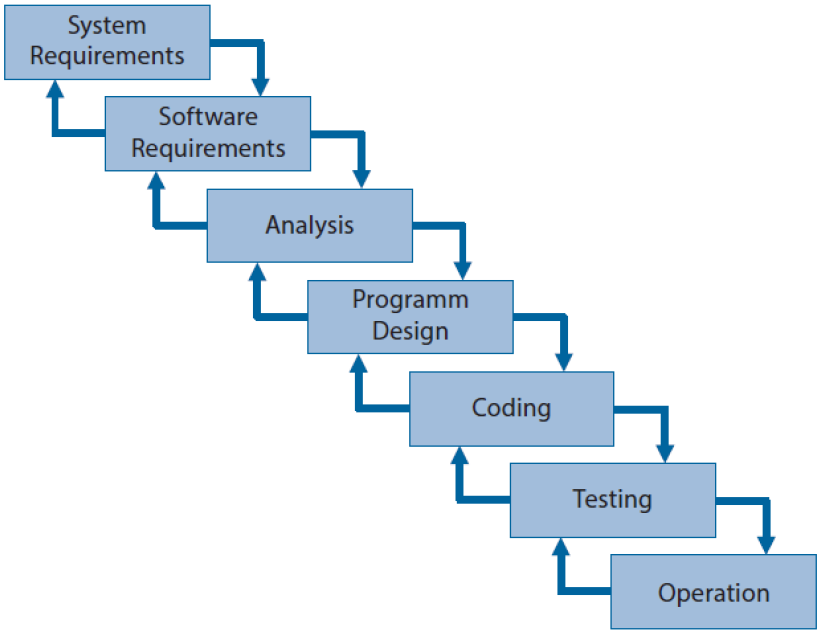
\includegraphics[width=150px]{img/Wasserfallmodell.png}
        \captionof{figure}{Das Wasserfallmodell}
        \label{fig:Wasserfallmodell}
\end{Figure}

Ebenfalls zu den sequentiellen Entwicklungsmodellen, gehört das V-Modell

\begin{Figure}
   \centering
    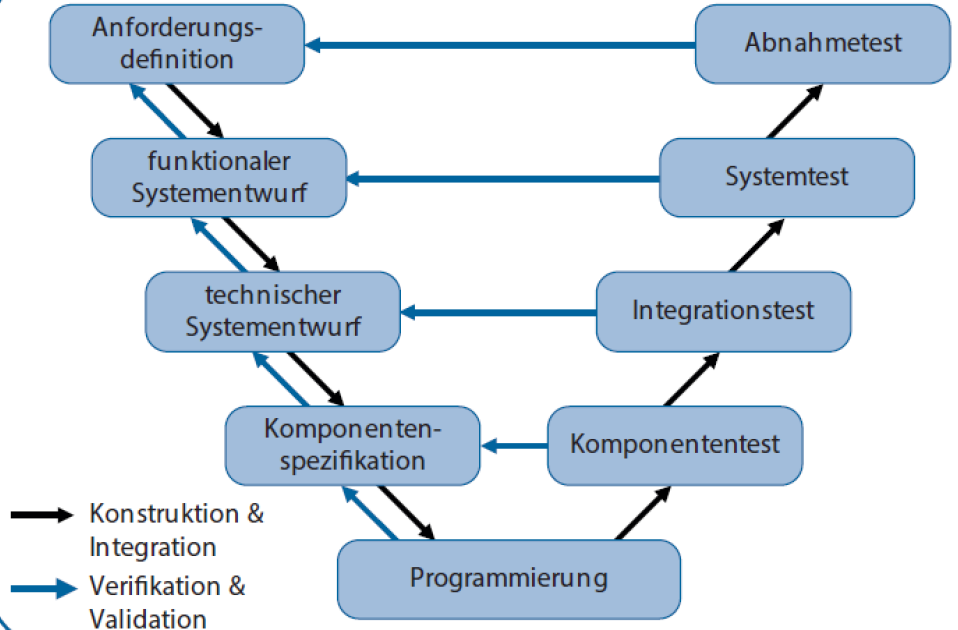
\includegraphics[width=150px]{img/VModell.png}
        \captionof{figure}{Das V-Modell}
        \label{fig:V-Modell}
\end{Figure}

Beim V-Modell trennt man den Konstruktions, mit den Testaktivitäten, sind jedoch gleichwertig aufzufassen (linke und rechte Seite). Dahingehend spricht man von arbeitsteiligen Teststufen, wobei jede Stufe 'gegen' ihre korrespondierende Entwicklungsstufe testet.\\

Dabei gibt es ein Sprachgebraucht nach ISTQB für das V-Modell
\begin{itemize}
   \item \textbf{Verifikation:} Bestätigung durch Bereitstellung eines objektiven Nachweises, dass festgelegte Anforderungen erfüllt worden sind ('Are we doing the thing right?')
   \subitem Alternative: Verfikation = formaler Korrektheitsbeweis 
   \item \textbf{Validierung:} Bestätigung durch Bereitstellung eines objektiven Nachweises, dass die Anforderungen für einen spez. beabsichtigten Gebrauch oder eine spezifische beabsichtigte Anwendung erfüllt worden sind ('Are we doing the right thing?')
   \subitem Alternative: Validierung = informelle Überprüfung 
\end{itemize}
$\rightarrow$ In der Praxis beinhaltet jeder Test beide Aspekte, wobei der validierende Teil mit steigender Teststufe zunimmt\\

Spricht man von testen innerhalb des Softwareentwicklungslebenszyklus:
\begin{itemize}
   \item Analyse und Entwurf der Tests während der Entwicklungsaktivtitäten
   \item Tester sollen im Review Prozess für Requirements oder Architektur als Stakeholder miteingebunden werden
\end{itemize}

\section{Iterative und inkrementelle Entwicklungsmodelle}
Die wohl bekannteste Form der iterativen Entwicklungsmodellen ist SCRUM.
\begin{Figure}
   \centering
    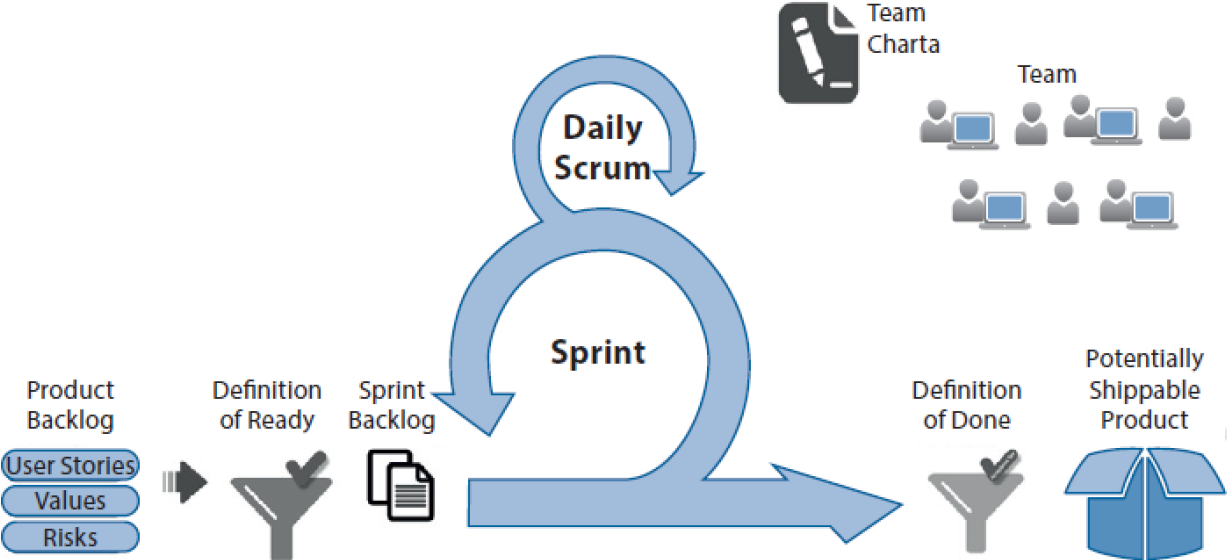
\includegraphics[width=150px]{img/Scrum.png}
        \captionof{figure}{Scrum}
        \label{fig:Scrum}
\end{Figure}
Dabei gibt es die \textbf{Testpyramide} nach Cohn und ist eine Hilfe für das Scrum-Team für die Überprüfung, ob die vorhandenen Testfälle angemessen und über sämtliche Teststufen verteilt sind.
\begin{Figure}
   \centering
    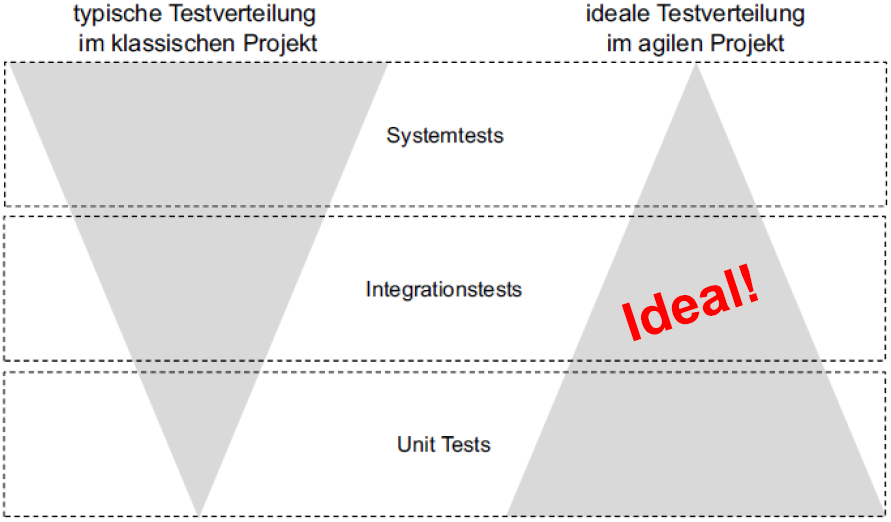
\includegraphics[width=150px]{img/Testpyramide.png}
        \captionof{figure}{Die Testpyramide nach Cohn}
        \label{fig:Die Testpyramide nach Cohn}
\end{Figure}

\subsection{Testmanagement in Scrum}
\begin{itemize}
   \item Ein Scrum-Team ist ein sich selbst organisierendes, interdisziplinäres Team
   \item Es gibt keinen Projektleiter, sondern vertraut darauf, dass ein Team sich selbst steuert
   \item Team ist gemeinsam für alle Arbeiten zuständig
   \item Programmierung und Testen ist nicht getrennt
   \item Testmgmt-Aufgaben existieren natürlich
   \item organisatorische Aufgaben fallen zum Scrum Master
   \item Leitungsaufgaben im Rahmen der Sprint-Planungspraktiken abgedeckt
   \item Testaufgaben entweder explizit über eigene Tasks oder implizit mit der Done-Kriterien anderer Aufgaben überwacht
   \item Testfortschritt und Testergebniss durch Continuous Integration ist hochautomatisiert
   \item CI kann durch Continuous Delivery erweitert werden $\rightarrow$ Wenn Tests fehlerfrei durchlaufen, wird es deployed
   \item klassische Testmanager wird überflüssig, jedoch nicht bei testfachlichen Aufgabenbereichen (Teststrategie und inhaltliches Planen)
   \item Gemäss Scrum würden diese Aufgaben allensamt mit dem Team durchgeführt
   \item Ein Teammitglied mit Testexpertise wird benötigt
   \item Mind. eine Person 'hauptamtlich' für das Testen zuständig sein
   \item Diese Person berät dann auch der PO bzgl. Produktqualität und Produktfreigabe
   \item Spricht nichts dagegen diese Person auch Testmanager im Scrum Team zu nennen
   \item auch exertne Testspezialisten sind öglich
   \item Auch in Scrum sind grundlegende klassische Testtechniken unverzichtbar
   \item Alle sollten geschult werden
   \item Scrum Master oder Testmanager müssten dafür sogar, dass diese Techniken umgeseztt werden
\end{itemize}


\section{Softwareentwicklung im Projekt- und Produktkontext}
Die Anforderungen an Planung und Nachvollziehbarkeit von Entwicklung undTest sind in unterschiedlichen Kontexten verschieden. Mögliche Punkte können eine Rolle spielen:
\begin{itemize}
   \item Geschäftsprioritäten
   \item Art des Produktes
   \item Markt- und technisches Umfeld
   \item Identifizierte Produktrisiken
   \item Organisatorische und kulturelle Aspekte
\end{itemize}
$\rightarrow$ Je nach Einsatzgebiet, sollen die Vorgehensmodelle angepasst werden (Tailoring)

\section{Teststufen}
Beim Testen kann und muss das zu testende System, seine Eigenschaften und sein Verhalten auch auf den versch. Ebenen der Architektur, von den elemanteren Einzelkomponenten bis zum Gesamtsystem, betrachtet und geprüft werden. 

Die Testaktivität einer solchen Ebene werden dabei als \textbf{Teststufe} bezeichnet. Jede Teststufe ist eine \textbf{Instanz des Testprozesses}. Nachfolgend werden die einzelnen Stufen im Detail betrachtet.

\subsection{Komponententest}
Komponenten werden isoliert getestet $\rightarrow$ Testen im Kleinen
\begin{itemize}
   \item Das Testobjekt beim Komponententest ist eine Komponente (Unit, Modul, Subsystem)
   \subitem Komponente sind ein Teil einer Applikation, bspw. eine Klasse oder Prozedur
   \subitem Keine Vorgabe über die Grösse einer Komponente
   \item Im Komponententest wird die Komponente an den Schnittstellen gegen die Spezifikation und das Softwaredesign getestet.
   \subitem es ist eine Komponente-Spezifikation erforderlich!  
   \item typische Testobjekte
   \subitem Komponenten, Klassen(-verbund)
   \subitem Programme
   \subitem Datenumwandlung / Migrationsprogramme
   \subitem Datenbankmodule
   \item Die Komponente sollte möglichst istoliert getestet werden
   \item Die Schnittstelle einer Komponente ist i.d.R. eine Programmierschnittstelle
   \item Wird ein Defekt gefunden, wird das i.d.R. der Komponente zugeordnet. 
\end{itemize}

\textbf{Testziele}
\begin{itemize}
   \item Test der Funktionalität
   \subitem Berechnungsfehler 
   \item Test auf Robustheit
   \subitem Durch Negativtests 
   \item Test der Effizienz
   \subitem Speicherverbrauch
   \subitem Antwortszeiten 
   \item Test auf Wartbarkeit (mittels statischer Analyse)
   \subitem Code-Kommentare
   \subitem Numerische Konstante 
\end{itemize}

\textbf{Testbasis:} 
\begin{itemize}
   \item Anforderung an die Komponente
   \item detaillierter Softwaredesign
   \item Code
\end{itemize}

\subsubsection{Teststrategie}

\textbf{Entwurfskriterien Testbarkeit}
\begin{itemize}
   \item Die Isolierbarkeit einer Komponente ist eine Voraussetzung für Komponententests
   \item Isolierbare Komponenten entstehen bei Entwurf nicht zwangsläufig - die Isoliebarkeit muss aktiv im Entwurf herbeigeführt werden
   \item Empfehlung: Testbarkeit sollte bei Entwurfsreviews mit einbezogen werden
\end{itemize}

\textbf{Test-First Ansatz}
\begin{itemize}
   \item Zuerst alle Testfälle implementieren und anschliessend produktiver Programmcode
   \item Stammt aus Extreme Programming (agile Methode)
   \item Vorteile
   \subitem QS der Anforderung
   \subitem Automatisierung spart Aufwand
   \subitem Test verliert den negativen beigeschmack
   \subitem Testfälle werden dokumentiert und sind reproduzierbar
   \item $\rightarrow$ In der Praxis stellt eine unvollständige Komponentenspezifikation ein grosses Problem dar! 
\end{itemize}

\subsection{Integrationstest}
Bildet die Brücke zwischen den Komponenten und dem Systemtest. Wobei als Integration die Verknüpfung der Komponenten zu grösseren Gruppen verstanden wird. \\

Der dazugehörige Integrationstest hat das Ziel, Fehlerzustände in den Schnittstellen und im Zusammennspiel zwischen integrierten Komponenten aufzudecken

\textbf{Testbasis}
\begin{itemize}
   \item Softwaredesign
   \item Systemdesign
   \item Systemarchitektur
   \item evtl. Workflows oder Use Cases
\end{itemize}

\textbf{Testobjekt}
\begin{itemize}
   \item Einzelbausteine zu grösseren Einheiten zusammenbauen
   \item Alle beteiligten Komponenten (inkl. Subsysteme, Externe Systeme und Datenbanken)
\end{itemize}

\textbf{Testumgebung}
\begin{itemize}
   \item Analog wie Komponententest
   \item Zusätzliche Monitore
   \subitem Mitschreiben von Datenbewegungen
   \subitem Standardmonitore für Protokolle
\end{itemize}

\textbf{Testziele}
\begin{itemize}
   \item Schnittstellen- und Protokollfehler aufdecken
   \subitem inkompatible Schnittstellenformate
   \subitem Untersch. Interpretation der übergegeben Daten
   \subitem Timing-Problem: Daten werden richtig übergeben aber zum falschen Zeitpunkt
\end{itemize}

\subsubsection{Integrationsstrategien}
\textbf{Top Down}
\begin{itemize}
   \item Der Test beginnt mit der Hauptkomponente
   \item Vorteil: Keine Testtreiber notwendig
   \item Nachteil: Noch nicht integrierte Komponenten müssen durch Platzhalter ersetzt werden
\end{itemize}

\textbf{Bottom Up}
\begin{itemize}
   \item Der Test beginnt mit der untersten Komponente
   \item Vorteil: Keine Platzhalter notwendig
   \item Nachteil: Übergeordnete Komponenten müssen durch Testtreiber simuliert werden
\end{itemize}

\textbf{Ad-Hoc}
\begin{itemize}
   \item Die Komponenten werden bspw. in der Reihenfolge ihrer Integration fertiggestellt
   \item Vorteil: Fertiggestellte Komponenten können zeitnah integriert werden
   \item Nachteil: Sowohl Testtreiber als auch Platzhalter sind erforderlich
\end{itemize}

\textbf{Backbone-Integration}
\begin{itemize}
   \item Es wird eine Programmskette (Backbone) erstellt, in das schrittweise die zu integrierende Komponente eingehängt werden
   \subitem Continuous Integration (CI) kann als moderne Realisierung dieser Integrationsstrategien gesehen werden
   \item Vorteil: Komponenten können in beliebiger Reihenfolge integriert werden
   \item Nachteil: Ein unter Umständen aufwendiger Backbone oder eine CI-Umgebung muss erstellt und gewartet werden
\end{itemize}

\textbf{Big Bang}
\begin{itemize}
   \item Der Test beginnt mit dem vollintegrierten System
   \item Vorteil: Es sind keine Testtreiber und Stubs notwendig
   \item Nachteil: Schwierige Fehlersuche - alle Fehlerwirkungen treten geballt auf
\end{itemize}

\subsection{Systemtest}
Test des Gesamtsytems $\rightarrow$ Kundensicht statt Entwicklersicht!

\begin{itemize}
   \item Test des Zusammenspiels aller integrierten Systemkomponenten
   \item Test in produktionsnaher Testumgebung
   \item Achtung: der Begriff System ist keinenfalls eindeutig definiertt
\end{itemize}

\textbf{Testbasis}
\begin{itemize}
   \item Alle DOkumenten die das Testobjekt auf Systemebene beschreiben wie Anforderungsdokumente, Spezifikation, Benutzungshandbücher etc.
\end{itemize}

\textbf{Testobjekt und Testumgebung}
\begin{itemize}
   \item Mit abgeschlossenem Integrationsstest liegt das komplett zusammengebaute Softwaresystem vor
   \item Systemgrenzen definieren
   \subitem Vor Systemtestbgeinng (besser vor Projektbeginn) ist diese Fragen genaustens zu kläre
\end{itemize}

\textbf{Testziele}
\begin{itemize}
   \item Validieren, ob und wie gut das fertige System die gestellten funktionalen und nicht-funktionalen Anforderungen erfüllt
   \item Fehler und Mängel aufgrund falsch, unvollständig oder im System widersprüchlich umgesetzter Anforderungen aufdecken
   \item Undokumentierte oder vergessenee Anforderungen identifizieren
   \item Prüfung der spezifizierten Systemeigenschaften
   \item Testen der nicht-funktionalen Anforderungen
\end{itemize}

\textbf{Probleme}
\begin{itemize}
   \item Testaufbau ist aufwändig
   \item (leicht vermeidbare) Fehler halten den Systemtest immer wieder auf
   \item Die Fehlerursache ist aufwändig zu finden
   \item Fehler können Schaden an der Betriebsumgebung anrichten (bspw. bei angeschlossenen Geräte)
\end{itemize}
$\Rightarrow$ Um Fehler zu finden ist der Systemtest der ungeeigeste Test. Man sollte die Fehler früher finden.

\subsection{Abnahmetest}
Spezieller Systemtest $\rightarrow$ Abnahme des Gesamt- oder Teilsystems durch Auftraggeber

\textbf{Mögliche Resultate}
\begin{itemize}
   \item Abnahmebescheinigung
   \item Nachbesserungsforderungen
   \item Rückgabe bzw. Minderung
\end{itemize}

\textbf{mögliche Formen}
\begin{itemize}
   \item Test auf vertragliche Konformität
   \item test der Benutzeraktzeptanz
   \item Akzeptanz durch den Systembetreiber
   \item Feldtest
\end{itemize}

\textbf{vertragliche Prüfung}
\begin{itemize}
   \item Der Kunde führt eine vertragliche Abnahme durch
   \item Basis der Ergebnisse entscheidet der Kunde ob das bestellte System den vertrg. Anforderungen entspricht
   \item Testkritieren sind im Entwicklungsvertrag beschriebenen Abnahmekriterien (können auch Normen oder gesetzliche Vorgaben sein)
   \item Abnahmeumgebung ist normalerweise die produktivumgebung des Kunden
\end{itemize}

\textbf{Test auf Benutzerakzeptanz}
\begin{itemize}
   \item User Acceptance Test (UAT)
   \subitem Akzeptanz jeder Anwendergruppen sicherzustellen
   \subitem Meinungen bzw. Bewertungen der Benutzer einholen
   \subitem Resultate sind oft nicht reproduzierbar
   \item mögliches Vorgehen: iterative-inkrementelle Entwicklung - Prototypen frühzeitig den Anwendern vorstellen 
\end{itemize}

\textbf{Akzeptanz durch den Systembetreiber}
\begin{itemize}
   \item Tests auf Passung in bestehenden IT-Infrastrukturen
   \subitem Backup, Wiederanlauf
   \subitem Benutzerverwaltung
   \subitem Aspekte der Datensicherheit
   \item Deployment-Test
   \item Test der Installierbarkeit
   \subitem Die für dieInstallation zugesicherten Installationsumgebung werden getestet
   \subitem virtuelle Umbgebung können den Aufwand zur Bereitstellung der nötigen Testumgebung deutlich reduzieren
   \item Update-Test
   \subitem Ähnlich Deployment Test
   \subitem Mögliche Ausgangsversionen sind zu berücksichtigen
   \item Test auf Deinstallierbarkeit
\end{itemize}

\textbf{Feldtest}
\begin{itemize}
   \item Bei Standardsoftware werden stabile Vorversion an einen ausgewählten Benutzerkreis ausgeliefert
   \subitem Alphatest
   \subitem Betatests
   \subitem Release Candidate
   \item Benutzer-Feedback muss organisiert sein
   \subitem User to Supplier
   \subitem Suppplier to User
\end{itemize}


\section{Testarten}
Folgende grundlegende Testarten lassen sich unterscheiden
\begin{itemize}
   \item Funktionale Tests und nicht-funktionale Tests
   \item Anforderungs- und strukturbasierte Tests
\end{itemize}
Wobei sich der Fokus und die Ziele je nach Stufe variieren. Dementsprechend kommen untersch. testarten in unterschd. Intesität zur Anwendung

\subsection{funktionale Tests}
\begin{itemize}
   \item Funktionalität beschreibt 'was' das System leisten soll (SOLL-Zustand)
   \item Funktionalität wird vom System, von einem Teilsystem oder einer Komponente geliefert
   \item Testbasis oder Referenz sind: Anforderungsspezifikation, Use Case, User Stories oder auch funktionale Spezfiikation
   \item funktionaler Test prüft das von aussen sichtbare Verhalten der Software (vgl. Blackbox Verfahren)
   \item Verwendung von spezifikationsbasierten Testentwurfsverfahren, um Testendekriterien und Testfälle aus der Funktionalität der SOftware /System herzuleiten
\end{itemize}

\subsection{nicht funktionale Tests}
\begin{itemize}
   \item nicht-funktionale Test prüft anhand von Software- und Systemmerkmalen 'wie gut' das System arbeitet
   \item Grundlagen gemäss Qualitätsmodelle (bspw. ISO 25010)
   \subitem Lasttest
   \subitem Performancetest
   \subitem etc.
\end{itemize}

\subsection{Anforderungsbezogener und strukturbezogener Test}
\begin{itemize}
   \item Anforderungsbezogenes Testen nutzt als Testbasis Spezfiikationen des extern beobachtbaren Verhaltens der Software
   \subitem Vorwiegend im System- und Abnahmetest eingesetzt
   \item strukturbezogenes Testen nutzt als Testbasis zusätzlich die interne Struktur bzw. Architektur der Software
   \subitem Vorwiegend im Komponenten- und INtegrationstest eingesetzt
   \subitem manchmal in höheren Stufen als Ergänzung  
\end{itemize}


\section{Test nach Änderung und Weiterentwicklung}
\begin{itemize}
   \item Jedes Softwaresystem bedarf über die Dauer seiner Nutzung gewisser Korrekturen und Ergänzungen
   \item In diesem Zusammenhang wird von Softwarewartung und Softwarepflege gesprochen
   \item Auslöser für die Änderungen eines Sofrwareprodukts sind die Korrektur von Fehlerzuständen oder die geplante Änderungen oder Ergänzungen einer Funktion
\end{itemize}

\subsection{Testen nach Softwarewartung und -pflege}
\begin{itemize}
   \item Falls Fehlerwirkung bewiesen, muss dieser beseitigt werden ($\rightarrow$ Fehlernachtest)
   \item Bei bereits getesteten Funktionalitäten muss bewiesen werden, dass kein Fehler vorliegt ($\rightarrow$ Regressionstest)
   \subitem Sind auch durchzuführen, wenn sich die Softwareumgebung ändert
   \item Nach- und Regressionstest werden oft mehrfach ausgeführt und müssen wiederholbar sein (Kandidaten für Testautomatisierung)
   \item Regressionstest umfassen funktionale, nicht-funktionale wie auch strukturelle Tests (auf allen Teststufen) 
\end{itemize}


\chapter{Statischer Test}
Testen von Software-Entwicklungsartefakten, ohne diese auszuführen, bspw. durch Reviews oder statische Analyse

\textbf{Reviews}
\begin{itemize}
   \item Manuelle Prüfungen durch eine oder mehr. Personen
   \item Menschliche Analyse- und Denkfähigkeit wird genutzt, um komplexe Sachverhalte zu prüfen und zu bewerten
   \item Kann bei allen Dokumenten durchgeführt werden, die während des Prozesses erstellt oder verwendet werden
\end{itemize}

\textbf{Statische (Code-) Analyse}
\begin{itemize}
   \item automatisierte Prüfung durch entsprschende Werkzeuge
   \item Nur bei Dokumenten mit formaler Struktur (bspw. Programmtext, UML-Diagramme etc.)
\end{itemize}

\section{Was kann analysiert und geprüft werden?}
\begin{itemize}
   \item Analyse des Testobjekts (Dokumente, Code etc.) durch intensive Betrachtung
   \item \textbf{Ziel:} Ermittlung von Fehlerzuständen (Defekten) im Dokument bzw. Code
   \subitem Verstösse gegen Spezifikationen, oder einzuhaltende Standards, Fehler in Anforderungen / im Design, falsche Schnittstellenspezifikation
   \subitem Nachweis der Verletzung von Projektplänen
   \subitem Ergebnisse der Untersuchungen werden darüber hinaus dazu benutzt, den Entwicklungsprozess zu optimieren
   \item \textbf{Grundidee:} Prävention
   \subitem Fehler(zustände) und Abweichungen sollen so früh wie möglich erkannt werden 
\end{itemize}

\section{Vorgehen}
Bei nicht-Werkzeuggestützten Verfahren $\rightarrow$ menschliche Analyse- und Denkfähigkeit verwenden. Dies erfolgt durch intensives Lesen und nachvollziehen, wobei Untersch. Verfahren, u.a. Review (von informell bis sehr formal) 
Entscheidung wann welches zum Tragen kommt, hat unterschiedliche Faktoren. 
\begin{itemize}
   \item Softwareentwicklungslebenszyklus-Modell
   \item Reife des Entwicklungsprozess
   \item Komplexität des zu überprüfenden Dokuments
   \item Gesetzliche oder regulatorische Anforderungen und / oder die Notwendigkeit eines Prüfnachweises (Audit-Trail)
\end{itemize}

\section{Reviewprozess}
Folgende Hauptaktvitäten gibt es bei einem Review
\begin{enumerate}
   \item Planung
   \item Initiierung, Kick-Off
   \item Indiv. Review
   \item Diskussion der Befunde
   \item Bericht und Fehlerbehebung
\end{enumerate}

\subsection{Planung}
\begin{itemize}
   \item Mgmt entscheidet welche Dokumente nach welcher Art einem Review unterzogen werden sollen
   \item entsprechender Aufwand ist einzuplanen
   \item Eingangs- und Austrittskriterien sind festzulegen
   \item Manager wählt Person für den Review aus und stellt ein Review-Team zusammen
\end{itemize}

\subsection{Initiierung (Kick-Off)}
\begin{itemize}
   \item Versorgung aller benötigten Informationen
   \item Überprüfung ob Eingangsbedingung erfüllt sind
   \item Schriftliche Einladung oder sofortiges erstes Treffen des Reviewteams
   \item Neben dem Arbeitsergebnis, müssen den beteiligten Personen weitere UNterlagen zur Verfügung gestellt werden:
   \subitem Dokumente, die herangezogen werden müssen um Review durchzuführen $\rightarrow$ Auch Basisdokumente (Baseline) bezeichnet
   \subitem Prüfkriterien (bspw. mit Checkliste) festlegen
   \subitem Sofern Vorlagen zur Protokollierung vorhanden, vorlegen
\end{itemize}

\subsection{Individuelles Review (indiv. Vorbereitung)}
\begin{itemize}
   \item beteiligte Personen müssen sich indiv. auf die Sitzung vorbereiten
   \item Reviewer setzen sich intensiv mit dem zu prüfenden Dokument auseinander
   \item Erkannte potentielle Fehler(zustände), Empfehlungen, Fragen oder Kommentare werden notiert
\end{itemize}

Beispiele für versch. indiv. Vorgehensweise:
\begin{itemize}
   \item Keine Vorgaben: ad-hoc-Vorgehen
   \item Strukturiertes Lesen: Vorgehen basiert auf Checklisten
   \item Strukturierte Richtlinie: Vorgehen unter Nutzung von Szenarien und Probeläufen $\rightarrow$ Dry Runs
   \item Prüfung aus einer Perspektive: Rollenbasiertes und perspektivisches Vorgehen
\end{itemize}

\subsection{Diskussion der Befunde (Reviewsitzung)}
\begin{itemize}
   \item Nach der indiv. Vorbereitung werden die Ergebnisse zusammengetragen und diskutiert
   \item Form: Reviewsitzung oder firmeninternen Onlineforum
   \item (potentielle) Abweichungen und Fehler(zustände) werden besprochen und näher analysiert
   \item Jedes Merkmale und das dazugehörige Ergebnis werden im Rahmen der Befundanalyse dokumentiert
   \item Reviewteam gibt eine Empfehlung über die Annahme (akzeptiert, Überarbeitung erforderlich, nicht akzeptieren) des Arbeitsergebnis ab
   \item Best-Practices
   \subitem max 2h Sitzung
   \subitem Moder hat das Recht, abzusagen oder abzubrechen
   \subitem Resultat und nicht Autor im Mittelpunkt
   \subitem Moderator darf nicht als Reviewer tätig sein
   \subitem Allg. Stilfragen dürfen nicht diskutiert werden
   \subitem Diskussion zur Lösung ist nicht Aufgabe des Reviewteams
   \subitem Jeder Reviewer muss die Gelegenheit haben, seine Befunde angemessen präsentieren zu können
   \subitem Ein Konses der Reviewer ist anzustreben und zu protokollieren
   \subitem Befunde nicht in Form von Korrekturanweisungen formulieren
   \subitem Befunde sind zu gewichten
\end{itemize}

\subsection{Bericht und Fehlerbehebung}
Ist die abschliessende Aktivität
\begin{itemize}
   \item Oftmals beinhaltet das Protokoll der Reviewsitzung alle erforderlichen Informationen
   \item Normalerweis behebt der Autor die Fehler(zustände)
   \item Die Reviewergebnisse können in Abhängigkeit von der Reviewart und dem Grad der Formalität stark variieren
\end{itemize}

\section{Rollen und Verantwortlichkeiten}

\subsection{Management}
\begin{itemize}
   \item Entscheidet über Durchführung von Reviews und deren Art
   \item Wählt die Prüfobjekte und die zu verwendenden Dokumente aus
   \item Verantwortlich für Planung und stellt die notwendigen Ressourcen (Personen, Budget, Zeit) zur Verfügung und das Review-Team zusammen
   \item Überwachung der Kosteneffizenz und das Treffen von steuernden Entscheidungen im Fall von unzureichenden Ergebnissen des Reviewprozesses
\end{itemize}

\subsection{Reviewleiter}
\begin{itemize}
   \item Reviewleiter trägt die Gesamtverantwortung für den Review (Planung, Vorbereitung, Durchführung und Über-/Nachbearbeitung)
   \item Entscheidet, welche Personen am Review beteiligt sind und organisiert Zeitpunkt und Räumlichkeit für Sitzung
\end{itemize}

\subsection{Reviewmoderator}
\begin{itemize}
   \item Leitet die Sitzung
   \item entscheidende Person für Erfolg
   \item Muss sehr guter Sitzungsleiter sein
   \item Muss bei gegensätzlichen Standpunkten vermitteln können und auch auf Untertöne achten
   \item Darf nicht voreingenommen sein und keine eigene Meinung zum Prüfobjekt äussern
\end{itemize}

\subsection{Autor}
\begin{itemize}
   \item Ersteller des Dokuments bzw. des Arbeitsergebnisses, das einem Review unterzogen wird
   \item Bei mehreren Erstellern sollte ein Hauptverantwortlicher benannt werden, der die Rolle des Autors übernimmt
   \item Wichtig ist, dass der Autor die geäusserte Kritik nicht als Kritik an seiner Person auffasst, sondern dass es ausschl. um die Verbesserung der Qualität geht
\end{itemize}

\subsection{Reviewer (Gutachter, Inspektor)}
\begin{itemize}
   \item Mehrere (max. 5) Fachexperten
   \item Verantwortung, gute Abschnitte entsprechend zu kennzeichnen
   \item Mangelhafte Teil zu dokumentieren und nachvollziehbar zu beschreiben
   \item Reviewer sollten gewählt werden, dass versch. Sichten im Reviewprozess vertreten sind
\end{itemize}

\subsection{Protokollant}
\begin{itemize}
   \item Dokumentiert alle Ergebnisse, Probleme und offene Punkte während Sitzung
   \item Kurz und präzise formulieren
   \item Schreibt Diskussionsbeiträge verfälschungsfrei auf
   \item Protokollant und Reviewmoderator sollte nicht dieselbe Person sein
   \item Manchmal sinnvoll, wenn der Autor auch der Protokollant ist
\end{itemize}

\section{Reviewarten}

\subsection{Informelles Review}
\begin{itemize}
   \item Abgeschwächte Form des Reviews
   \item Autor-Leser-Feedbackzyklus
\end{itemize}

\subsection{Walkthrough}
\begin{itemize}
   \item Mittelpunkt eine Sitzung
   \item kein formaler Ablauf
\end{itemize}

\subsection{technische Review (auch fachliches Review)}
\begin{itemize}
   \item Übereinstimmung des Prüflings mit einer Spezifikation, Eignung für den Einsatz, Einhaltung von Standards
   \item Hinzuziehen von Fachexperten
\end{itemize}

\subsection{Inspektion}
\begin{itemize}
   \item Formalste Art
   \item definierter Ablauf mit genauen Prüfkriterien
   \item Aufdeckung von Unklarheiten, mögliche Fehler(zustände), Bestimmung der Qualität, Vertrauen in das Arbeitsergebnis schaffen
\end{itemize}


\section{Erfolgsfaktoren, Vorteile und Grenzen}
\begin{itemize}
   \item Reviews sind effiziente Mittel zur Sicherung der Qualität
   \item Idealerweise direkt nach Fertigstellung der Arbeitsergebnisse durchzuführen
   \item Frühe Finden von Fehler(zustände)n durch Reviews meist kostengünstiger als das spätere Erkennen
   \item Wissensaustausch unter den beteiligten Personen
   \item Organisatorische Erfolgsfaktoren
   \subitem Mgmt und PL unterstützen Reviews
   \subitem angemessene Frist geplant
   \subitem genügend Zeit für Vorbereitung
   \subitem Checklisten sind aktuell
   \subitem Umfangreiche Dokumente werden nicht als ganzes geprüft
   \item Personenbezogene Erfolgsfaktoren
   \subitem passende Personen auswählen
   \subitem dienen zur Qualitätssicherung
   \subitem ausreichend Zeitnehmen und Aufmerksamkeit für Details
   \subitem Kultur des 'ständigen Lernens'
\end{itemize}

\section{Unterschied statische vs. dynamische Tests}
\begin{itemize}
   \item Statische und dynamische Tests können das gleiche Ziel verfolgen $\rightarrow$ Fehler finden
   \item statische Tests entdecken Fehler direkt in Dokumente
   \item dynamische Tests weisen Fehlerwirkungen nach - vor allem im Programmcode und nicht in anderen Dokumenten
\end{itemize}

\section{Statische (werkzeugbasierte) Analyse}
Oftmals Oberbegriffe für alle Prüfverfahren, bei denen keine Ausführung des Testobjekts erfolgt
\begin{itemize}
   \item Überprüfung, Vermessung und Darstellung eines Dokuments bzw. eines Programms oder einer Kopmonente
   \item müssen formale Struktur haben
   \item typischerweise wird Quelltext analyisert
   \item Prüfung auf Einhaltung von Konventionen und Standards
   \item Datenflussanalyse
   \item Kontrollflussanalyse
   \item Erhebung von Metriken
\end{itemize}
Als Beispiel ist der Compiler zu nennen

\subsection{Prüfung der Einhaltung von Konventionen und Standards}
\begin{itemize}
   \item Einhaltung der Programmierkonventionen durch Analysatoren
   \item Möglichst automatisch überprüfen lassen
\end{itemize}

\subsection{Datenflussanalyse}
\begin{itemize}
   \item ur-Anomalie: Ein undefinierter Wert (u) einer Variablen wird auf einem Programmpfad gelesen (r)
   \item du-Anomalie: Die Variable erhält einen Wert (d), der allerdings ungültig (u) wird, ohne dass er zwischenzeitlich verwendet wurde
   \item dd-Anomalie: Die Variable erhält auf einem Programmpfad ein zweites Mal einen Wert (d), ohne dass der erste Wert (d) verwendet wurde
\end{itemize}
Bspw. mit SonarLint oder SpotBugs

\subsection{Kontrollflussanalyse}
\begin{itemize}
   \item Programmstück kann als Kontrollflussgraph dargestellt werden
   \item Anweisung + Sequenz von Anweisung ist ein Knoten
   \item Änderungen werden durch Verzweigungen und Schleifen erreicht
   \item Durch die Visualisierung der Kontrollflussgraphen lassen sich Anomalien leicht erfassen
   \subitem Sprünge aus Schleifen
   \subitem Mehrere Ausgänge
\end{itemize}

\subsection{Ermittlung von Metriken}
\begin{itemize}
   \item Werkzeuge der statischen Analyse liefern auch Messwerte (Siehe ISO DIN 25010)
   \item Werkzeuge: SonarQube, Eclipse Metrics
\end{itemize}

\subsection{Zyklomatische Zahl}
\begin{itemize}
   \item die Zyklomatische Zahl oder Komplexität misst die sturkturelle Komplexität des Quellcodes
   \item Grundlage für die Berechnung ist der Kontrollflussgraph
   \item Die zyklomatische Zahl kann genutzt werden, um Abschätzungen in Bezug auf die Testbarkeit und die Wartbarkeit des Programmteils vorzunehmen
   \item Zahl höher als 10 ist nicht tolerabel $\rightarrow$ 3-6 ist akzeptabel
   \item Zahl gibt Auskunft über den Testaufwands
   \item Zyklomatische Zahl = Anzahl linear unabhängigen PFade im Programmstück $\rightarrow$ obere Grenze für die benötigten Testfälle zur Erreichung dieses Kriteriums
\end{itemize}

\end{document}